\documentclass[a4paper, 12pt]{article}
\usepackage[utf8]{inputenc}
\usepackage[english,russian]{babel}
\usepackage[warn]{mathtext}
\usepackage{graphicx}
\usepackage{float}
\usepackage{multirow}
\restylefloat{table}
\usepackage{amsmath}
\usepackage{floatflt}
\usepackage[T2A]{fontenc}
\usepackage[left=20mm, top=20mm, right=20mm, bottom=20mm, footskip=10mm]{geometry}

\tolerance 1414
\hbadness 1414
\emergencystretch 1.5em
\hfuzz 0.3pt        % размер максимального переполнения без warning'a
\widowpenalty=10000 % запрещает одиночную строку абзаца в начале страницы
\vfuzz \hfuzz
\raggedbottom       % если на странице мало содержимого, добавить пустое место в конце, а не в середине страницы



\begin{document}

\begin{titlepage}
	\centering
	\vspace{5cm}
	{\scshape\LARGE московский физико-технический институт (национальный исследовательский университет) \par}
	\vspace{6cm}
	{\scshape\Large Лабораторная работа 8.1 \par}
	{\huge\bfseries Тепловое излучение \par}
	\vspace{1cm}
	\vfill
\begin{flushright}
	{\large Б03-104}\par
	\vspace{0.3cm}
	{\LARGE Куланов Александр}
\end{flushright}
	

	\vfill


	Долгопрудный, 2023 г.
\end{titlepage}

\begin{itemize}
	\item \textbf{Цель работы:} При помощи модели абсолютно черного тела провести измерения температуры оптическим пирометром с исчезающей
	нитью и термопарой, исследовать излучение накаленных тел с различной испускательной способностью, определить постоянные планка и Стефана-Больцмана.
\end{itemize}

\section{Теоретические сведения}
Для измерения температуры разогретых тел, удаленных от наблюдателя, применяют методы оптической пирометрии, основанные на использовании зависимости испускательной способности исследусмого тела от температуры. Различают три температуры, функционально связанные с истинной термодинамической температурой и излучательной способностью тела: радиационную $T_{\text {рад }}$, цветовую $T_{\text {нв }}$ и яркостную $T_{\text {ярк }}$.

Под радиационной (энергетической) температурой понимают температуру абсолютно черного тела, при которой его интегральная испускательная способность одинакова с интегральной испускательной способностью исследуемого тела.

Под цветовой температурой исследуемого тела понимают температуру абсолютно черного тела, при которой отношение их спектральных испускательных способностей для двух заданных длин волн одинаково.

Под яркостной температурой понимают температуру абсолютно черного тела, при которой его спектральная испускательная способность равна спектральной испускательной способности исследуемого тела при той же длине волны. Именно эту температуру мы будем измерять в данной работе.

Измерение яркостной температуры раскаленного тела производится при помощи оптического пирометра с исчезающей нитью, основанного на визуальном сравнении яркости раскаленной нити с яркостью изображения исследуемого тела. Равенство видимых яркостей, наблюдаемых через монохроматический светофильтр $(\lambda=6500 A)$, фиксируется по исчезновению изображения нити на фоне раскаленного тела. Яркостный метод измерения температуры основан, в соответствии с формулой Планка, на зависимости испускательной способности абсолютно черного тела от температуры и длины волны.

Оптический пирометр представляет собой зрительную трубу, внутри которой имеется накаливаемая нить, расположенная в плоскости изображения исследуемого раскаленного тела, а также темно-красный светофильтр $(\lambda=6500 A)$. Через окуляр одновременно наблюдается изображение исследуемого тела и раскаленной нити.

Если в том узком спектральном интервале, который пропускается светофильтром, яркость нити меньше яркости раскаленного тела, то нить видится темной полоской на светлом фоне, и наоборот. При совпадении яркостей нить перестает быть видимой на фоне изображения раскаленного тела. Регулировка яркости нити осуществляется изменением тока, протекающего через нее.

Шкалу прибора, измеряющего ток через нить, предварительно градуируют по абсолютно черному телу, термодинамическую температуру которого измеряют с помощью термопары. Если тело, температуру которого определяют, излучает как абсолютно черное тело, то мы можем с помощью пирометра найти его температуру. Если же тело излучает иначе, то определенное значение температуры является яркостной температурой. Яркостная температура тела всегда ниже его термодинамической температуры. Это связано с тем, что любое нечерное тело излучает меньше, чем абсолютно черное тело при той же температуре. Чтобы получить величину термодинамической температуры тела, надо вводить дополнительные поправки, которые определяются для каждого материала экспериментально. В данной работе используется оптический пирометр с исчезающей нитью, проградуированный при изготовлении по абсолютно черному телу, так что его цифровое табло во время измерения высвечивает значение температуры накаленного тела в градусах Цельсия. Вначале
с помощью модели абсолютно черного тела проверяется правильность работы пирометра, а затем с его помощью исследуется излучение различных материалов и вольфрамовой нити накаливания. Необходимая для обработки проводимых в данной работе измерений зависимость между яркостной и термодинамической температурами вольфрама приведена на рис. 1.

\begin{figure}[H]
    \centering
    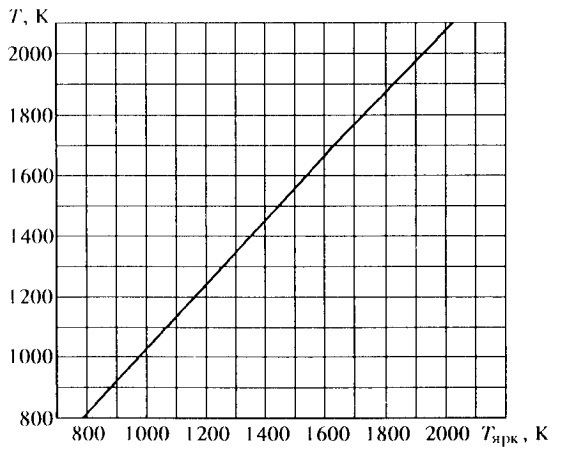
\includegraphics[width=0.5\textwidth]{tunsgten.jpg}
    \caption{График зависимости термодинамической температуры от яркостной температуры для вольфрама}
    \label{fig:tungs}
\end{figure}


По результатам измерений мощности излучения вольфрамовой нити можно судить о справедливости закона Стефана-Больцмана. Для этого следует мощность, потребляемую нитью, приравнять к излучаемому ею за единицу времени количеству энергии. Если бы нить излучала как абсолютно черное тело, то баланс потребляемой и излучаемой энергии определялся бы соотношением
\begin{equation}
W=\sigma S\left(T^4-T_0^4\right),
\end{equation}

где $W$ - потребляемая нитью электрическая мощность, $S-$ площадь излучающей поверхности нити, $T$ - температура нити, $T_0$ температура окружающей среды. Однако вольфрамовая нить излучает как нечерное тело. Среди нечерных тел выделяются так называемые серые тела, для которых характер распределения излучения совершенно подобен спектру абсолютно черного тела, но излучение ослаблено по сравнению с ним в $\varepsilon_T$ раз для любой длины волны при данной температуре тела $T$.

Если предположить, что нить излучает как серое тело, то выражение (1) можно записать в виде
\begin{equation}
W=\varepsilon_T S \sigma T^4,
\end{equation}
где мы учли, что реально температура вольфрама намного выше температуры окружающей среды. Значения коэффициента излучения $\varepsilon_T$ при различных температурах приведены на рис. 2.

\begin{figure}[H]
    \centering
    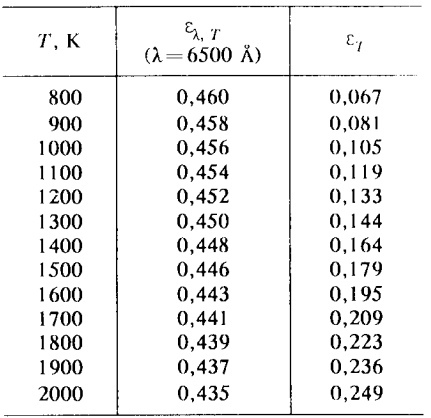
\includegraphics[width=0.5\textwidth]{tabl1.jpg}
    \caption{Поправочные коэффициенты излучения для вольфрама}
    \label{fig:tabl}
\end{figure}

\section{Экспериментальная установка}

Схема установки представлена на рисунке (\ref{fig:set})

\begin{figure}[H]
    \centering
    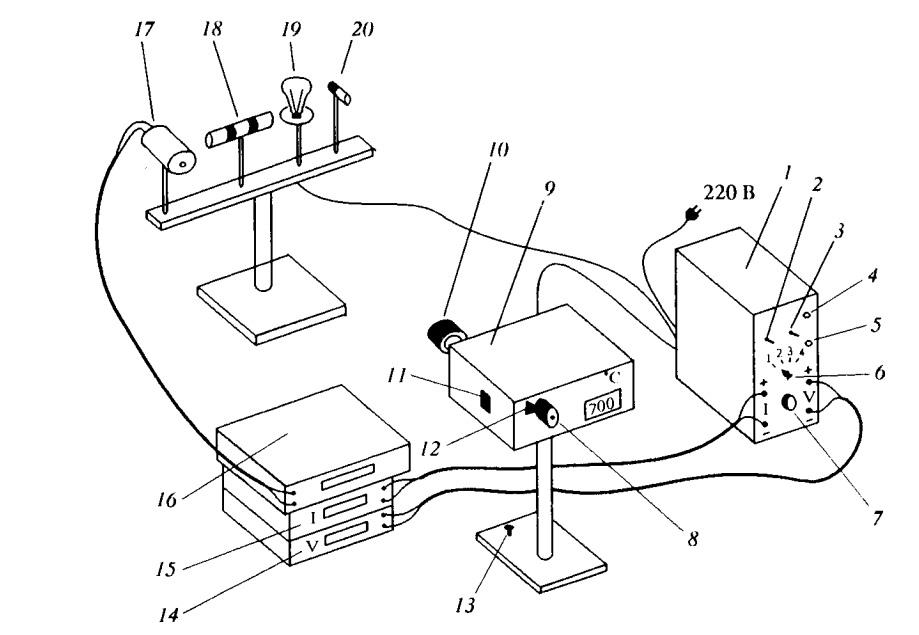
\includegraphics[width=0.7\textwidth]{set.jpg}
    \caption{Схема установки}
    \label{fig:set}
\end{figure}
1 - блок питания; 2 - тумблер включения питания пирометра и образцов; 3 - тумблер нагрева нити пирометра: «Быстро» - вверх, «Медленно - вниз; 4 - кнопка «Нагрев нити»; 5 - кнопка *Охлаждение нити; 6 - тумблер переключения образцов; 7 - регулятор мощности нагрева образцов; 8 - окуляр пирометра; 9 - корпус пирометра; 10 - объектив пирометра; 11 - переключение диапазонов: $700-1200^{\circ} \mathrm{C}$ - вниз, $1200-2000^{\circ} \mathrm{C}$ - вверх; 12 - сектор красного светофильтра; 13 - регулировочный винт; 14 - вольтметр (напряжение на лампе накаливания); 15 - амперметр (ток через образцы); 16 - вольтметр в цепи термопары; 17 - модель АЧТ; 18 - трубка с кольцами из материалов с разной излучательной способностью; 19 - лампа накаливания; 20 - неоновая лампочка


\section{Обработка результатов}
\subsection*{Проверка работы оптического пирометра}
В этой части работы сравним температуру модели АЧТ, измеренную при помощи термопары и пирометра.
\begin{table}[H]
	\centering
	\begin{tabular}{|l|l|l|l|l|}
	\hline
	U, В                      & 41.0 & 34.8 & 35.9 & 37.1 \\ \hline
	Темп. по пирометру, град. & 1060 & 900  & 931  & 959  \\ \hline
	Темп. по термопаре, град  & 1010 & 855  & 880  & 910  \\ \hline
	Отклонение, \%             & 4.7  & 5.0  & 5.4  & 5.1  \\ \hline
	\end{tabular}
\end{table}
Как мы видим, отклонение составило порядка 5\%, что, в общем, в пределах нормы для этой работы.
\subsection*{Измерение яркостной температуры раскаленных тел}
В этой части работы можем наблюдать, что при одинаковой термодинамической температуре, равной в нашем случае 900 градусам, яркостная температура колец разная.
Это различие связано с тем, что кольца сделаны из разных материалов, которые не явяются АЧТ. У них разные коэффициенты поглощения.
\subsection*{Провекра закона Стефана-Больцмана}
Измерим пирометром яркостную температуру нити, силу тока и напряжение через каждые 100 градусов. 
\begin{table}[H]
	\centering
	\begin{tabular}{|l|l|l|l|l|l|l|l|l|l|l|}
	\hline
	$T_\text{ярк}$ & 910   & 1000  & 1100  & 1200  & 1300  & 1400  & 1500  & 1600  & 1700  & 1800  \\ \hline
	U, В           & 1.605 & 1.976 & 2.359 & 2.916 & 3.390 & 3.892 & 5.374 & 5.824 & 7.531 & 8.618 \\ \hline
	I, A           & 0.507 & 0.547 & 0.587 & 0.640 & 0.684 & 0.729 & 0.849 & 0.882 & 1     & 1.073 \\ \hline
	$T$            & 920   & 1020  & 1130  & 1240  & 1345  & 1450  & 1560  & 1670  & 1780  & 1890  \\ \hline
	\end{tabular}
\end{table}
Для каждого значения найдем термодинамическую температуру вольфрамовой нити
лампы из графика, приведенного ранее. Для проверки закона Стефана-Больцмана построим график зависимости $W = \varepsilon_T B T^n$ в лог. масштабе, т. е.
\begin{equation}
	\ln W = \ln (\varepsilon_T B) + n \ln T
\end{equation}
Коэффициент наклона прямой должен быть близок к 4. Построим ради интереса график той же функции, но полагая $T = T_\text{ярк}$
\begin{figure}[H]
    \centering
    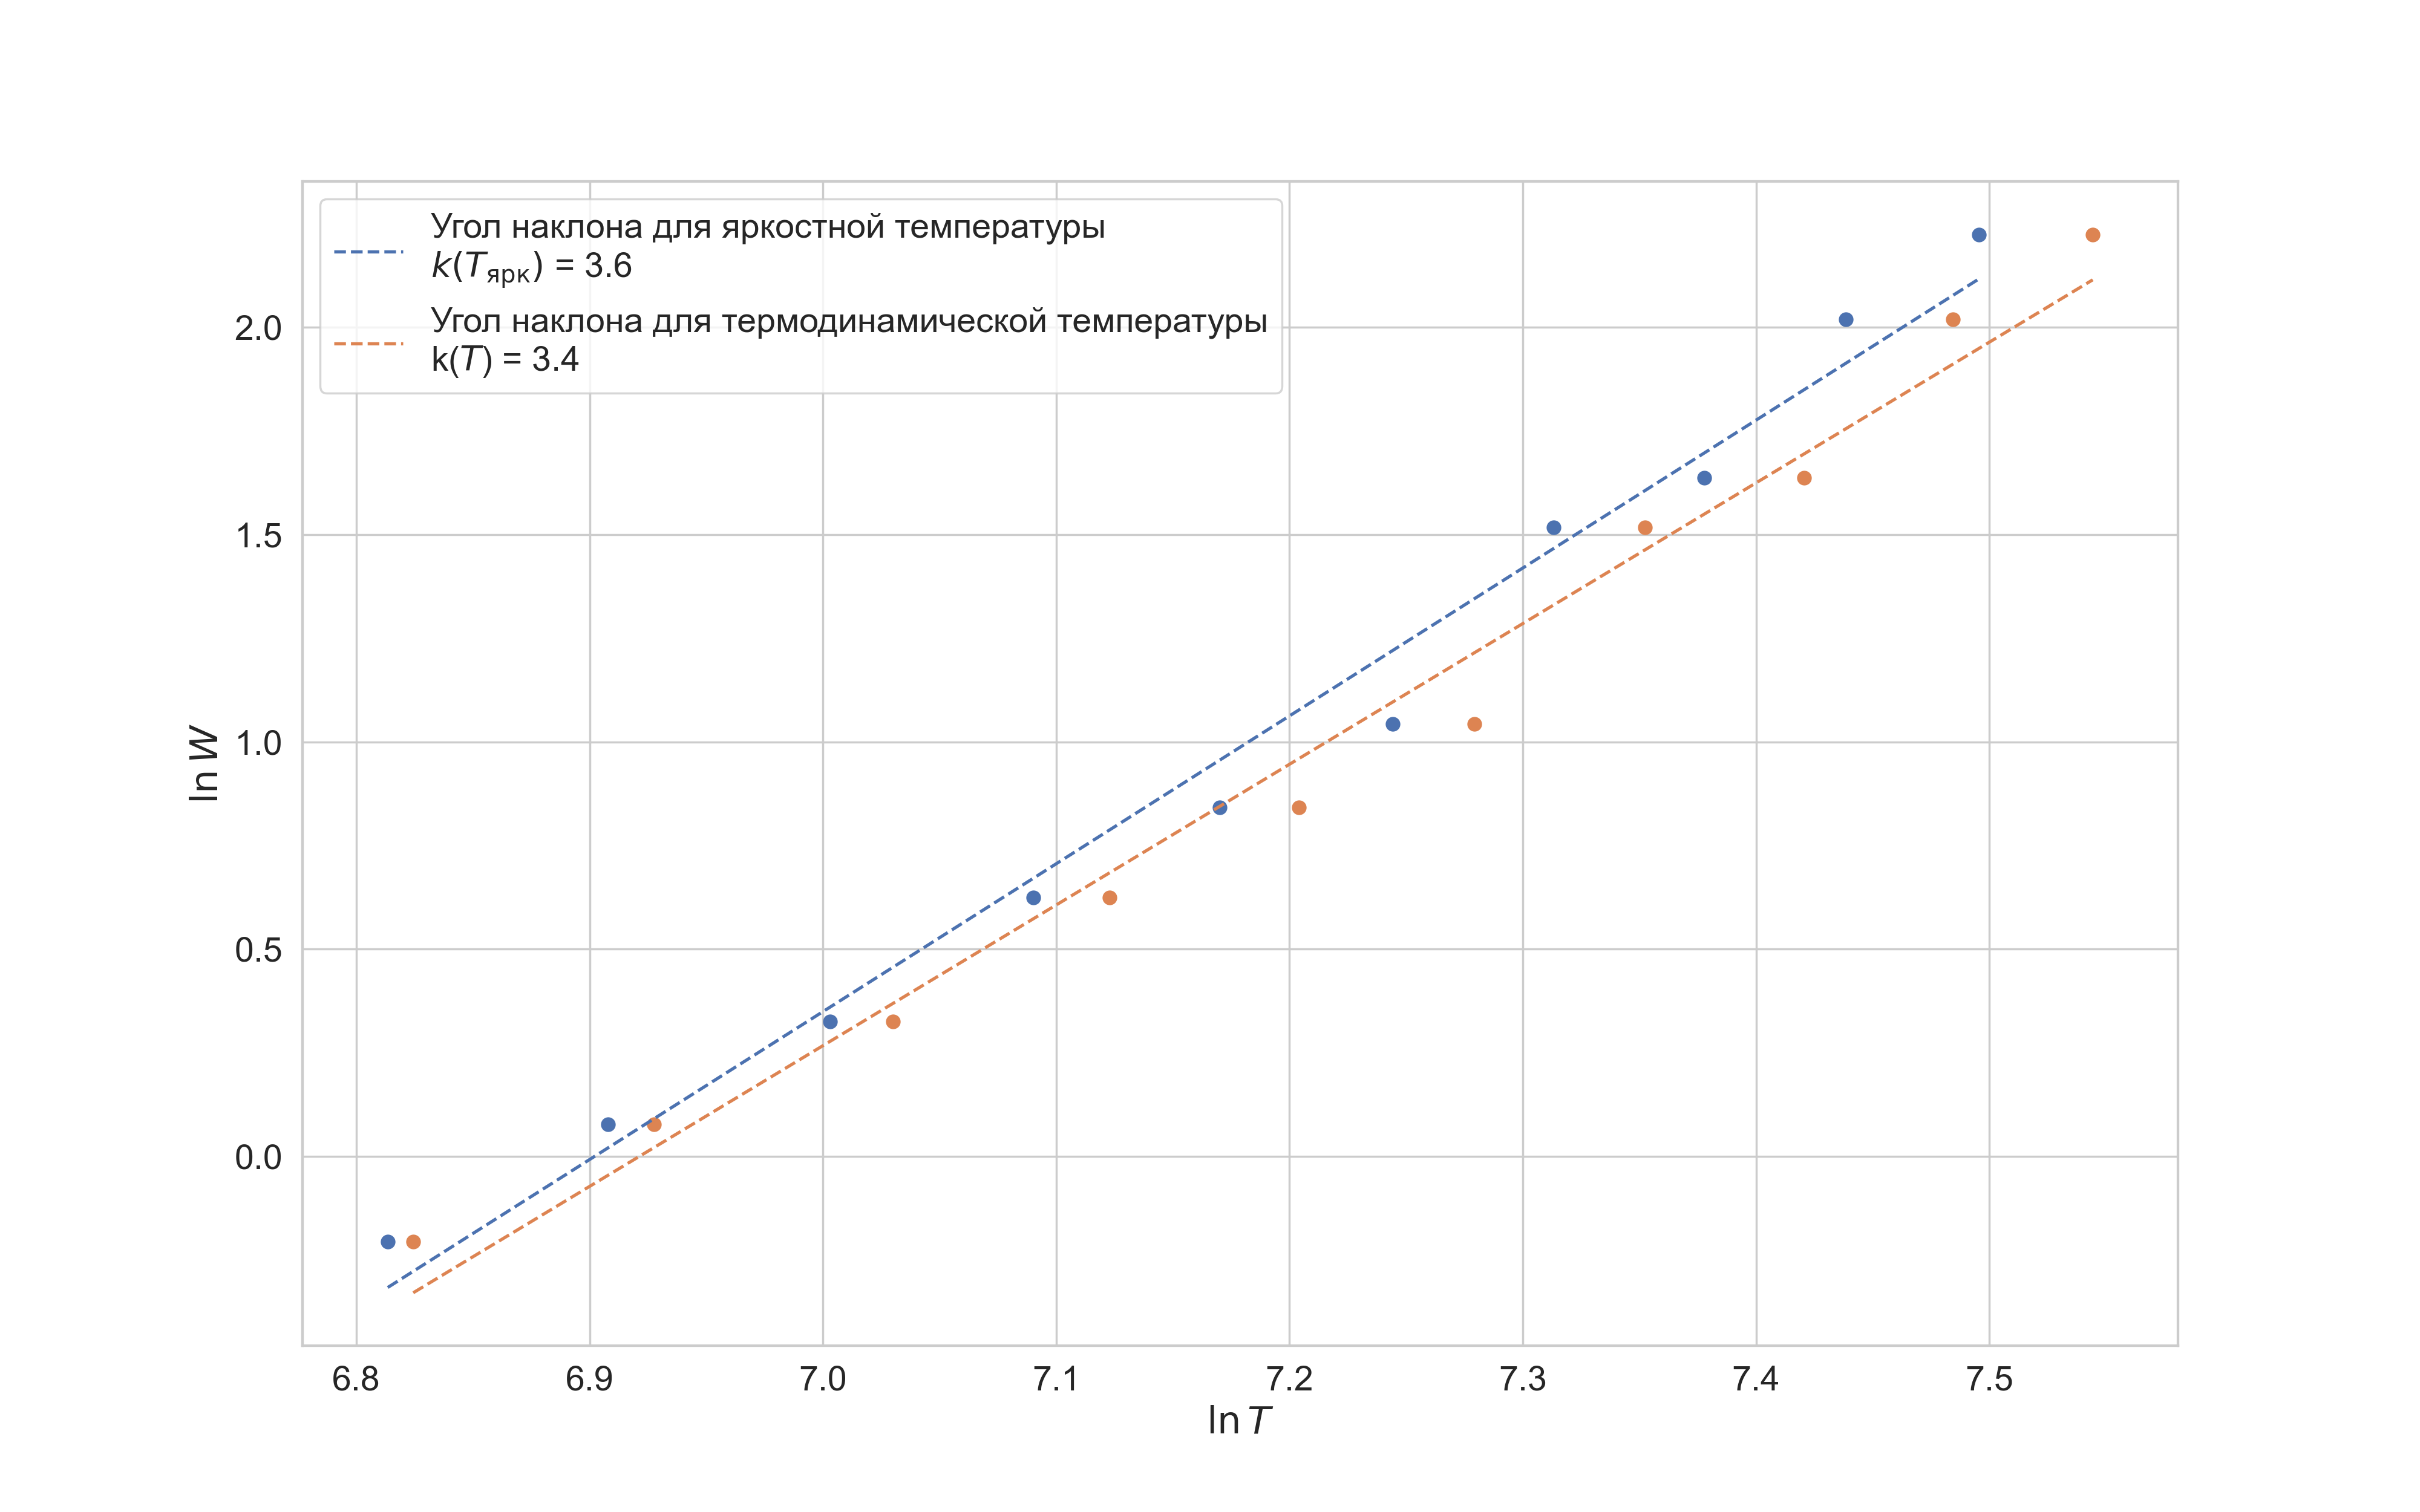
\includegraphics[width=1\textwidth]{plotLog.png}
    \caption{Зависимость $\ln W = f(\ln T)$}
    \label{fig:plotlog}
\end{figure}
Получили для термодинамической температуры наклон $3.4 \pm 0.1$, а для яркостной $3.6 \pm 0.1$. Это говорит о том, что график пересчета температур неверен.
Найдем величину постоянной Стефана-Больцмана по формуле
\begin{equation}
	\sigma = \frac{W}{\varepsilon_T S T^4}
\end{equation}
где $T = 1973 K$, $S = 0,36 \text{ см}^2$, $\varepsilon_T \approx 0,244$ (из таблицы), $W = 7,531 \text{ Вт}$. Получаем 
\begin{equation*}
	\sigma = (5,66 \pm 0.03)\cdot 10^{-12} \frac{\text{Вт}}{\text{см}^2\text{К}^4}
\end{equation*}
Это хорошо совпадает с теоретическим значением, равным
\begin{equation*}
	\sigma_{theor} = 5,67\cdot 10^{-12}\frac{\text{Вт}}{\text{см}^2\text{К}^4}
\end{equation*}
Оценим значение постоянной планка:
\begin{equation*}
	h = \sqrt[3]{\frac{2 \pi ^5 k_b^4}{15 c^2 \sigma}} \approx 6,6 \text{ Дж}\cdot \text{с}
\end{equation*}
\subsection*{Яркостная температура неоновой лампы}
Термодинамическая температура лампы порядка комнатной, в то время как яркостная - порядка 900 градусов. Такое отличие связано с тем, что неоновая не является моделью АЧТ или серого тела, и излучает в связи с переходами электронов между энергетическими уровнями.

\section{Выводы}
В ходе работы было изучено тепловое излучение модели АЧТ и серых тел. Был исследован закон Стефана-Больцмана: получили $W \propto T^{3,6}$. Это может быть связано с разными факторами: теплоотвод от нити, ошибки в определении яркости. 

Была оценена постоянная Стефана-Больцмана. Значение сошлось с теоретическим в пределах погрешности. Также была оценена постоянная Планка.

Кроме того, было показано, что термодинамическая температура вообще не обязана совпадать с яркостной на примере неоновой лампы.

\end{document}